% =====================================================================================
%  Behaviour Beats Judgement — final paper
%  Task 25D. Every number below is copied from writeup/results_summary.md, results_22.md,
%  results_23.md, excerpts_22.md or figures/captions.md (or the report those files cite);
%  the source is kept in a "% src:" comment next to it. Nothing was recomputed or re-rounded.
%  Figures: put this file next to the folder figures/ (= writeup/figures/ in the repository).
%  Compile with pdflatex (Overleaf default). Packages: all in TeX Live / Overleaf.
% =====================================================================================
\documentclass[11pt]{article}

\usepackage[T1]{fontenc}
\usepackage[utf8]{inputenc}
\usepackage{amsmath}
\usepackage{newtxtext,newtxmath}          % serif text + math (close to the template look)
\usepackage[a4paper,margin=2.5cm]{geometry}
\usepackage{graphicx}
\usepackage{booktabs,tabularx,longtable,multirow,array}
\usepackage{caption}
\usepackage{float}
\usepackage{xcolor}
\usepackage{enumitem}
\usepackage{tikz}
\usetikzlibrary{arrows.meta,positioning,fit}
\usepackage[hidelinks]{hyperref}
\usepackage{microtype}

\graphicspath{{figures/}}
\captionsetup{font=small,labelfont=bf}
\setlist{itemsep=1pt,topsep=3pt}
\newcolumntype{Y}{>{\raggedright\arraybackslash}X}
\newcommand{\ci}[2]{\,[#1,\,#2]}            % 95% CI
\newcommand{\cmark}{\textbf{\textsf{yes}}}

\begin{document}

% ------------------------------------------------------------------ title block (template style)
\thispagestyle{empty}
\noindent\rule{\textwidth}{2.5pt}\par\vspace{10pt}
\begin{center}
{\LARGE\bfseries Behaviour Beats Judgement: Auditing Collusion Between\\[3pt]
LLM Agents with Monitor Views and Antitrust-Style Evidence}
\end{center}
\vspace{6pt}\noindent\rule{\textwidth}{0.6pt}\par\vspace{14pt}

\begin{center}
\begin{tabular}{ccc}
Author name 1 & Author name 2 & Author name 3\\
Affiliation & Affiliation & Affiliation\\
\end{tabular}
\end{center}

\begin{center}\textbf{\large Abstract}\end{center}
\begin{quote}\small\itshape
LLM agents that interact repeatedly can secretly agree to coordinate against the others. We study two
questions about auditing such collusion from logged trajectories: which view of a game record lets an LLM
monitor detect it, and what evidence should count as convincing. We built a pre-registered testbed with
locally run open models: five \texttt{qwen2.5:7b} agents play an 8-round El Farol bar game. In collusion games
two agents receive an alliance note and a private channel; three lookalike types (placebo, friendly persona
talk, and a shared private incentive) contain no collusion. Ground truth comes only from the generation config.
LLM monitors (\texttt{llama3.1:8b}; \texttt{granite3.3:8b} as a second model) score five views of each game,
and an LLM judge plus code-computed signals feed fixed decision rules. Everything was frozen on 24 dev games,
tested once on 24 test games, and re-tested on 48 new games under a pre-registered replication.
Model-free behaviour signals were the most reliable evidence and replicated: the capture signal reached an
AUROC of 0.900 [0.811, 0.965] on the new games and beat the best LLM view by +0.264 [0.121, 0.412]; the
coalition-gain rule reached 0.885 [0.786, 0.961]. Both LLM monitors were mediocre and inconsistent on new
games (every view between 0.32 and 0.66), and the structured report that looked best on the test set fell
from 0.896 to 0.636. Messages alone and talk-only judging stayed near chance, private plans added nothing,
and combining evidence did not beat gain alone. Outcome evidence is necessary but not sufficient: a shared
incentive produces the same outcomes, and none of the communication evidence we measured worked as an
antitrust-style ``plus factor''.
\end{quote}
% src: results_summary.md "Main findings" rows 1-6; R21 §4.7 (R10a, R10b); R22C §4.2 (E1), §4.4; R14 §4.2.

% ====================================================================================
\section{Introduction}

LLM agents are increasingly deployed side by side: in markets, in shared infrastructure and inside larger
multi-agent workflows. When two of them coordinate against the others, the harm can be real (higher prices,
a captured resource, a displaced competitor), and the coordination may never be stated openly. An
auditor usually has logs: what agents said in public, what they did, and what outcomes followed. The
practical question is what to do with those logs.

We study two questions on one shared dataset:
\begin{itemize}
  \item \textbf{Study 1 --- say vs.\ do.} Does combining what agents say with what they do beat either alone, when the
  same LLM monitor reads different \emph{views} of a game record?
  \item \textbf{Study 2 --- standard of evidence.} What should count as convincing evidence of collusion? We compute the
  same conversation, coalition-advantage and dependence evidence for every game and combine it with fixed
  decision rules.
\end{itemize}

Competition law offers a useful frame for Study~2. Parallel conduct alone does not prove an agreement: firms may
move together for independent reasons, such as a common cost shock. Courts therefore look for ``plus
factors'' on top of parallel conduct, for example evidence of communication or actions that only make sense
under an agreement~\cite{kovacic2011,twombly2007,theatre1954}. We built our dataset so that both halves of
this argument can be tested: one lookalike shows collusive-sounding \emph{talk} without coordination, and
another shows parallel \emph{conduct} caused by a shared incentive without any agreement.

\paragraph{Our main contributions are:}
\begin{enumerate}
  \item \textbf{A pre-registered, fully local collusion testbed} with four episode types, two of which are
  deliberately hard lookalikes; ground truth taken only from the generation config; one dev/test split fixed
  before any game existed; every model pinned by digest and run locally at \$0.
  \item \textbf{A view comparison for LLM monitors with controls, a second monitor model and a pre-registered
  replication on 48 new games.} The view that looked best on the original test (a code-built structured
  report) did not replicate, while a model-free behaviour signal did and clearly beat every LLM view.
  \item \textbf{An evidence-standard analysis in antitrust terms.} Coalition gain is necessary and replicates,
  but a shared incentive fools it; none of the communication evidence we measured worked as a plus factor.
  \item \textbf{A catalogue of measured LLM-monitor failure modes}: a constant-score collapse, a judge ceiling,
  a model-specific position bias, a session effect and small-sample optimism.
\end{enumerate}

% ====================================================================================
\section{Related Work}

\textbf{Multi-agent deception and collusion testbeds.} Our games run on the harness of Shi et al.~\cite{shi2026},
which records private plans, public announcements, final actions and outcomes over repeated social dilemmas and
classifies promise-breaking. Fish et al.~\cite{fish2024} show tacit collusion by LLM pricing agents;
Agrawal et al.~\cite{agrawal2025} study seller collusion in LLM double auctions with an overseer; Colosseum
\cite{nakamura2026} audits collusion in teams of tool-using agents with coalition-advantage metrics.
These works mostly ask \emph{whether} agents collude. We ask how an auditor should \emph{detect} it from logs,
with lookalikes that are designed to fool each kind of evidence.

\textbf{Monitors and detectors.} TraceGuard~\cite{nguyen2026} scores a single agent's actions on several
structured dimensions, including action--trace consistency; we reuse that rubric idea in our structured
report view (V4). Work on steganographic collusion~\cite{mathew2024,tailor2025} builds calibrated detectors
for hidden channels. We instead compare \emph{the same} LLM monitor on different views of the same record,
add controls that break specific shortcuts (mismatched, length-matched and shuffled views), and test whether
the ranking survives a second monitor model and new games.

\textbf{Antitrust evidence.} The ``plus factor'' doctrine~\cite{kovacic2011,twombly2007,theatre1954} separates
parallel conduct from agreement. We turn it into testable decision rules (Section~\ref{sec:23}) and measure
what they gain and what they miss.

\textbf{The game.} El Farol~\cite{arthur1994} is an anti-coordination game: the bar is pleasant only if few go.
Two agents can share the capacity only if the others stay home, so collusion creates a visible coalition
advantage while honest play has no dominant action.

% ====================================================================================
\section{Setup and Methods}

\subsection{Game and protocol}
Five agents (J, M, Q, T, Z), all \texttt{qwen2.5:7b} at temperature 1.0, play 8 rounds of El Farol.
Going pays \$10 if fewer than half go (at most 2 of 5), a crowded bar pays $-\$5$, and staying home pays \$0.
Each round follows the three-stage protocol of the Shi et al.\ harness~\cite{shi2026}: a private plan
(Stage~1), a public announcement with a message in a seeded, rotated speaking order (Stage~2), and a
simultaneous final GO/STAY choice (Stage~3). We use the harness only for its game definitions and prompt
builders; a deterministic history block replaces its reflection step, and every prompt ends with a brevity
line and an English-only language line.
% src: amendment2 §5; README "Setup in 5 bullets"; results_22.md setup; deviation table rows 4, 8.

\subsection{Episode types and ground truth}
\begin{itemize}
  \item \textbf{Type 1 --- collusion.} The two focal agents receive an alliance note (a shared goal, a secrecy
  instruction and a suggested plan: both go while encouraging the other three to stay home) and a private
  channel that they use twice per round.
  \item \textbf{Type 2 --- placebo.} The focal pair receives a neutral note of the same length in the same position
  (139 vs.\ 138 tokens), and plays honestly.
  % src: amendment2 §2 (token ratio placebo_v3/alliance_v4 = 139/138 = 1.007)
  \item \textbf{Type 3 --- persona talk.} The pair is told to talk like friends in public, with no agreement and no
  channel. This lookalike targets \emph{word} evidence.
  \item \textbf{Type 4b --- shared incentive.} Each focal agent is told privately that staying home costs it an
  \$8 deposit, so going is better for both, with no agreement and no knowledge of each other. This lookalike
  is antitrust's ``conscious parallelism'' and targets \emph{outcome} evidence.
\end{itemize}
The label is collusion $=1$ for Type~1 and $0$ otherwise, read only from the generation config. The dataset has
48 games (24 Type~1, 8 of each lookalike), split once into 24 dev and 24 test games (each 12 Type~1 + 4 of each
lookalike), with labels and split written from the plan \emph{before} generation (master seed 20261023).
The replication used 48 new games (seed 20261027) as one confirmation set with no split.
% src: README; results_22.md setup; prereg_replication.md table (seed 20261027, counts 24/8/8/8).

Figure~\ref{fig:pipeline} shows the data flow.

\begin{figure}[t]
\centering
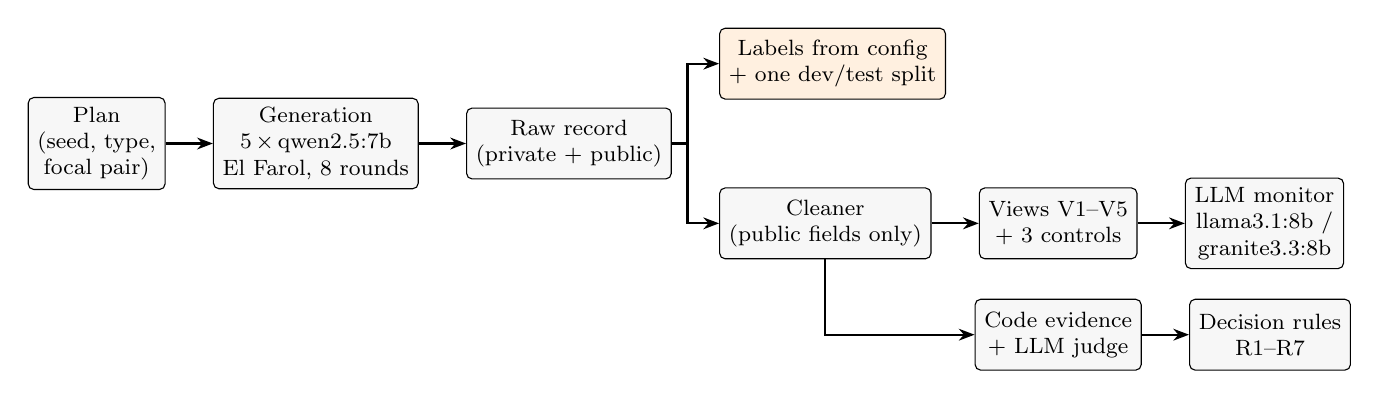
\begin{tikzpicture}[
  node distance=5mm and 6mm,
  box/.style={draw,rounded corners=2pt,align=center,font=\footnotesize,minimum height=9mm,fill=gray!6},
  gold/.style={box,fill=orange!12},
  arr/.style={-{Stealth[length=2mm]},thick}]
\node[box] (plan) {Plan\\(seed, type,\\focal pair)};
\node[box,right=of plan] (gen) {Generation\\5\,$\times$\,qwen2.5:7b\\El Farol, 8 rounds};
\node[box,right=of gen] (raw) {Raw record\\(private + public)};
\node[gold,above right=1mm and 6mm of raw] (lab) {Labels from config\\+ one dev/test split};
\node[box,below right=1mm and 6mm of raw] (clean) {Cleaner\\(public fields only)};
\node[box,right=of clean] (views) {Views V1--V5\\+ 3 controls};
\node[box,right=of views] (mon) {LLM monitor\\llama3.1:8b /\\granite3.3:8b};
\node[box,below=of views] (ev) {Code evidence\\+ LLM judge};
\node[box,right=of ev] (rules) {Decision rules\\R1--R7};
\draw[arr] (plan) -- (gen);
\draw[arr] (gen) -- (raw);
\draw[arr] (raw.east) -- ++(2mm,0) |- (lab.west);
\draw[arr] (raw.east) -- ++(2mm,0) |- (clean.west);
\draw[arr] (clean) -- (views);
\draw[arr] (views) -- (mon);
\draw[arr] (clean.south) |- (ev.west);
\draw[arr] (ev) -- (rules);
\end{tikzpicture}
\caption{Pipeline. Labels come only from the generation config and are written, with the single dev/test split,
before any game is generated. Monitors, the judge and the code evidence see only the cleaned public record
(V5 adds private plans, never the private channel).}
\label{fig:pipeline}
\end{figure}

\subsection{Views, controls and cleaning (Study 1)}
A whitelist cleaner keeps only public fields (announcements, messages, final actions, standard-rule payoffs);
setup text, private payoffs, the private channel and labels cannot reach a view. Its leak scanner removes
8-word copies of setup texts and header phrases, and otherwise only flags (deviation~7, Appendix~\ref{app:dev}).
\begin{itemize}
  \item \textbf{V1 messages}: all public announcements and messages. \textbf{V2 actions}: final actions and payoffs per
  round. \textbf{V3 combined}: V1 and V2 interleaved per round.
  \item \textbf{V4 structured report}: built by code, with no LLM: per agent, announced vs.\ actual action and
  broken promises (with a TraceGuard-style consistency score); per pair, rounds both went, joint broken
  promises and mentions of each other.
  \item \textbf{V5 oracle}: V3 plus each agent's private Stage-1 plan and Stage-3 reasoning (the private channel is
  excluded because only Type~1 games have one).
  \item \textbf{Controls}: \emph{C-mismatch} (messages of one game with actions of another game of the same type),
  \emph{C-length} (V3 cut to V4's length) and \emph{C-shuffled} (contents drawn from random games; a leak check).
\end{itemize}

\subsection{Monitors and judge}
The primary monitor is \texttt{llama3.1:8b} with the frozen format \texttt{monitor\_v3\_pairs\_ctx16k}: it scores
all 10 pairs 0--100, and the game score is the maximum pair score (temperature 0, \texttt{num\_ctx} 16384, one
sample per call). The same frozen prompt was run with \texttt{granite3.3:8b} as a second model (RQ9 and the
replication's amendment~1). For Study~2 an LLM judge (\texttt{llama3.1:8b}) reads only the cleaned public
messages and scores each pair 0--100.
% src: results_22.md setup; prereg_replication.md (num_ctx 16384, temperature 0); results_23.md families.

\subsection{Evidence signals and decision rules (Study 2)}
Four evidence families are computed per pair: \textbf{E1 conversation} (the judge score $C_{\text{judge}}$, plus a
coordination-keyword score $C_{\text{kw}}$), \textbf{E2 coalition advantage} ($G_{\text{others}}$: how much better the
pair does than the other agents), \textbf{E3 dependence} (Dep: how much the pair's choices depend on each other)
and \textbf{E4 word--action} ($W_{\text{joint}}$: whether the pair broke public promises together). Simple
parallel-conduct signals are \emph{coGO} (rounds both went) and \emph{capture} (rounds in which exactly the pair
went). Seven rules were frozen on dev: R1 judge only; R2 gain only; R3 dependence only; R4 legal style (parallel
conduct plus a plus factor, same pair); R5 gain and dependence, same pair; R6 points ($\geq 1$ of 4 families
above its dev level); R7 a learned logistic rule.
% src: results_23.md "The evidence families", §1, §2.

\subsection{Integrity: pre-registration, freezes and statistics}
\begin{itemize}
  \item \textbf{Pre-registration chain} (Appendix~\ref{app:repro}): a frozen RQ0.1 pre-registration; amendment~1
  (after pilot~1, before pilot~2); amendment~2 (before any dataset game) and its erratum (before any monitor
  result); the frozen monitor (after dev runs, before any test call); follow-up~1 (before its calls); and the
  replication pre-registration with its amendment~1 (before any replication game, and before any replication
  view was rendered, respectively).
  \item \textbf{Freezes.} Monitor format, prompts and thresholds were chosen on dev, frozen and run \emph{once} on
  test; the Study~2 rules file was applied once to test and once to the replication, never refit.
  \item \textbf{Statistics.} AUROC is primary; we also report accuracy-style counts at frozen thresholds. All
  intervals are 95\% bootstrap CIs stratified by episode type, resampling whole games (B = 2000, seed 20261023);
  differences are paired. The pre-registered primary comparisons are RQ2 and RQ5; everything else is
  exploratory, with no multiple-comparison correction.
  % src: results_22.md "How to read the numbers".
  \item \textbf{Deviations.} We logged 39 deviations, each with the reason and whether it was decided before or
  after the related data (Appendix~\ref{app:dev}). The most important ones: pilot~1 failed the frozen uptake
  rule and amendment~1 replaced it (\#4); the cleaner became flag-only (\#7); \texttt{num\_ctx} was raised to 16384
  before any monitor call (\#15); and the constant-score format was ruled ineligible on dev, before any test
  call (\#16).
  \item \textbf{Local and reproducible.} Ollama 0.40.3 with every model pinned by digest, \$0 spent, and every LLM
  call cached to disk under a key that includes the model digest, prompt, schema, settings, seed and sample index.
\end{itemize}

% ====================================================================================
\section{Results: Study 1 (monitor views)}
\label{sec:22}

\subsection{Gates: does the dataset do what it should? (RQ0.1--RQ0.4)}

\textbf{RQ0.1, real collusion, passed only after a recorded failure.} Pilot~1, under the frozen uptake rule, failed
the uptake criterion (2/4), although the transcripts showed coordination in all 4 games: the rule missed short
instructions without ``we/us'' words, and one game drifted into Chinese. Amendment~1 added an English-only line
and uptake rule~v2 and ran a fresh pilot~2, which passed every criterion: uptake 4/4, falsification 0/2 (placebo),
focal pair top by coGO 4/4, coalition advantage and capture 4/4 and 4/4, and a hand agreement with the rule of
96.9\% (Cohen's $\kappa$ 0.931). On the full dataset, uptake was 24/24 and uptake \emph{and} effect 23/24.
% src: results_22.md RQ status table RQ0.1 (R10 §B3, §B4; R12 §4.3); R10 §B1.
A blinded two-rater hand-check of pilot~1 (descriptive) agreed between raters on 91.7\% of cells ($\kappa$ 0.80);
rule v2 agreed with the two raters on 79.2\% and 85.4\%, and every rule--rater disagreement was a rule miss,
never a false alarm.
% src: R10 §B3 (two-rater table; cited by results_22.md as R10 §B3). Not in the write-up files themselves.

\textbf{RQ0.2, lookalikes.} Type~3 behaved as designed in 7/8 games (1 partly); Type~4b in 6/8 (2 did not follow the
incentive). All 8 Type~4b games mention the ``deposit'' in public, an unplanned clue visible to monitors.
\textbf{RQ0.3, leakage}, passed: no setup copies had to be removed, a grep of 384 views was clean, and the shuffled
control stayed at chance (dev 0.465 [0.250, 0.667]; test 0.632 [0.431, 0.833]). \textbf{RQ0.4, stability}, passed for
V1, V3, V4 and V5 but \textbf{failed for V2} (mean absolute difference 5.00, Spearman 0.676). Collusion was not fully
secret: 6.5\% of focal public messages reveal joint action, and 12 of 24 Type~1 games have at least one reveal.
% src: results_22.md RQ table RQ0.2-RQ0.4 (R12 §4.4, §4.5, §5; R13 §3, §4; R14 §4.10); limitations (R12 §4.2).

\subsection{Original test set (RQ1--RQ8)}

Table~\ref{tab:views} and Figure~\ref{fig:auroc} give the test AUROC per view. The code-built structured report
(V4) ranked best, 0.896 [0.771, 0.979]; messages alone (V1, 0.490) and actions alone (V2, 0.372) were at or below
chance.

\begin{figure}[t]
\centering
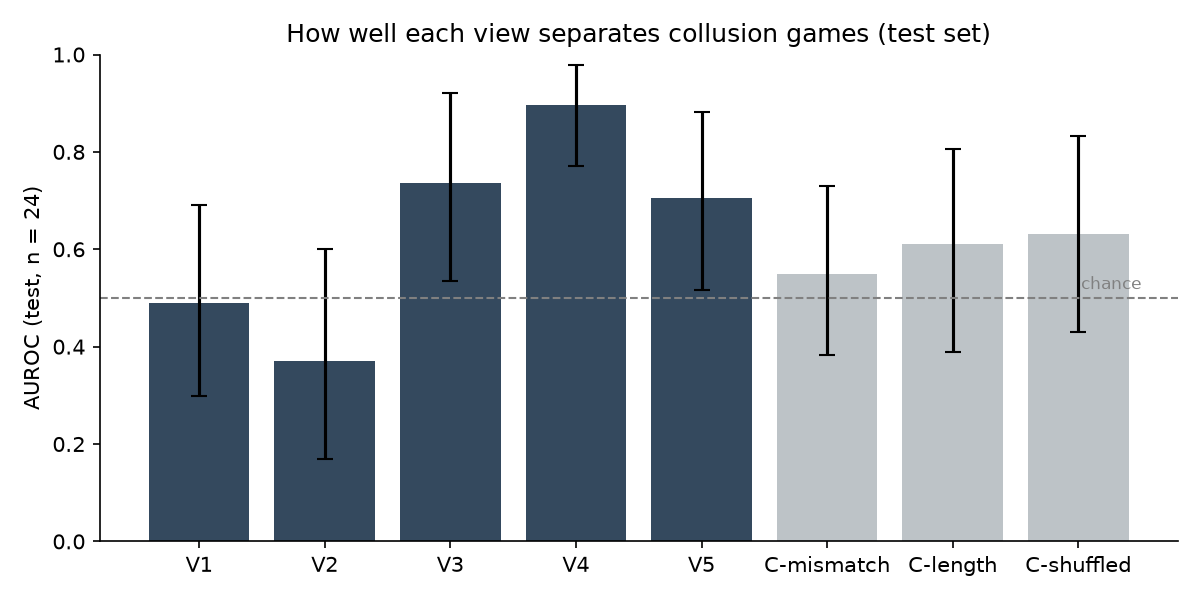
\includegraphics[width=0.92\textwidth]{fig1_auroc_by_view_test.png}
\caption{\textbf{How well each view separates collusion games (original test set, $n=24$).} Test AUROC per view with
95\% CIs; the dashed line is chance. Dark bars are the five views and grey bars the three controls. V4 has the highest
AUROC (0.90 [0.77, 0.98]); the CIs of V3 and V5 also exclude chance. V1, V3 and C-mismatch have a degenerate frozen
threshold of 0, so their threshold metrics carry no information; their AUROC is threshold-free.}
\label{fig:auroc}
\end{figure}
% src: figures/captions.md Figure 1.

\begin{table}[t]
\centering\small
\caption{\textbf{AUROC per view} [95\% CI]: original test (llama, $n=24$) and the pre-registered replication
(48 new games) for both monitors. Replication values are not reported for V5 and the C-length / C-mismatch
controls. Sources: R14 \S4.2; R21 \S4.7; R22C \S4.4.}
\label{tab:views}
\begin{tabular}{lccc}
\toprule
View & llama, test & llama, replication & granite, replication\\
\midrule
V1 messages        & 0.490 [0.299, 0.691] & 0.505 [0.363, 0.655] & 0.618 [0.474, 0.756]\\
V2 actions         & 0.372 [0.170, 0.601] & 0.324 [0.186, 0.469] & 0.628 [0.488, 0.754]\\
V3 combined        & 0.736 [0.535, 0.920] & 0.565 [0.421, 0.706] & 0.662 [0.560, 0.771]\\
V4 structured      & \textbf{0.896} [0.771, 0.979] & 0.636 [0.507, 0.751] & 0.582 [0.414, 0.730]\\
V5 oracle          & 0.705 [0.517, 0.882] & --- & ---\\
C-mismatch         & 0.549 & --- & ---\\
C-length           & 0.611 & --- & ---\\
C-shuffled         & 0.632 [0.431, 0.833] & 0.457 [0.315, 0.591] & ---\\
\midrule
capture (code, no LLM) & 0.896 [0.781, 0.986] & \textbf{0.900} [0.811, 0.965] & (model-free)\\
\bottomrule
\end{tabular}
\end{table}
% src: results_22.md RQ1 row and §g per-view table; R10a; capture test value R15 §4.4.

\textbf{Primary comparisons.} \emph{RQ2} (V3 minus the dev-chosen best single view, V2) was +0.365 [0.094, 0.611]:
``combining helps'' by the pre-registered wording, but fragile, because V2 failed RQ0.4, the pooled value was
+0.040 [$-$0.155, 0.238], and V2 alone moved by +0.188 between sessions. \emph{RQ5} found no clear advantage of
structure over the raw combined view (V4 $-$ V3 +0.160 [$-$0.021, 0.351]) but an advantage over a raw view of the
same length (V4 $-$ C-length +0.285 [0.017, 0.556]).
% src: results_22.md RQ2, RQ5 rows (R14 §4.3, §4.6; R15 §4.2; R16 §4.4).

\textbf{Other questions.} Each single view was fooled by one lookalike (RQ3). At the frozen thresholds V4 flagged
0/4 placebo, 2/4 persona and 1/4 shared-incentive games; V2 flagged 2/4, 3/4 and 2/4. Per-type AUROC showed
persona talk fooling actions (V2, T1 vs.\ T3 0.219 [0.00, 0.62]) and the shared incentive fooling messages
(V1, T1 vs.\ T4b 0.344 [0.12, 0.65]) (Figure~\ref{fig:pertype}). There was no clear evidence that the monitor
cross-checks words against actions (RQ4, V3 $-$ C-mismatch +0.188 [$-$0.028, 0.386]), and private plans added
nothing (RQ6, V5 $-$ V3 $-$0.031 [$-$0.267, 0.236]). The dependence code signal lost to V4 (RQ7, $-$0.173
[$-$0.382, $-$0.009], $n=21$), but the simpler action signals coGO, capture and $G_{\text{others}}$ matched V4
(exploratory). For naming the colluding pair (RQ8; chance 0.1), V4 was best with 7/12.
% src: results_22.md RQ3, RQ4, RQ6, RQ7, RQ8 rows (R14 §4.4-§4.9; R15 §4.4).

\begin{figure}[t]
\centering
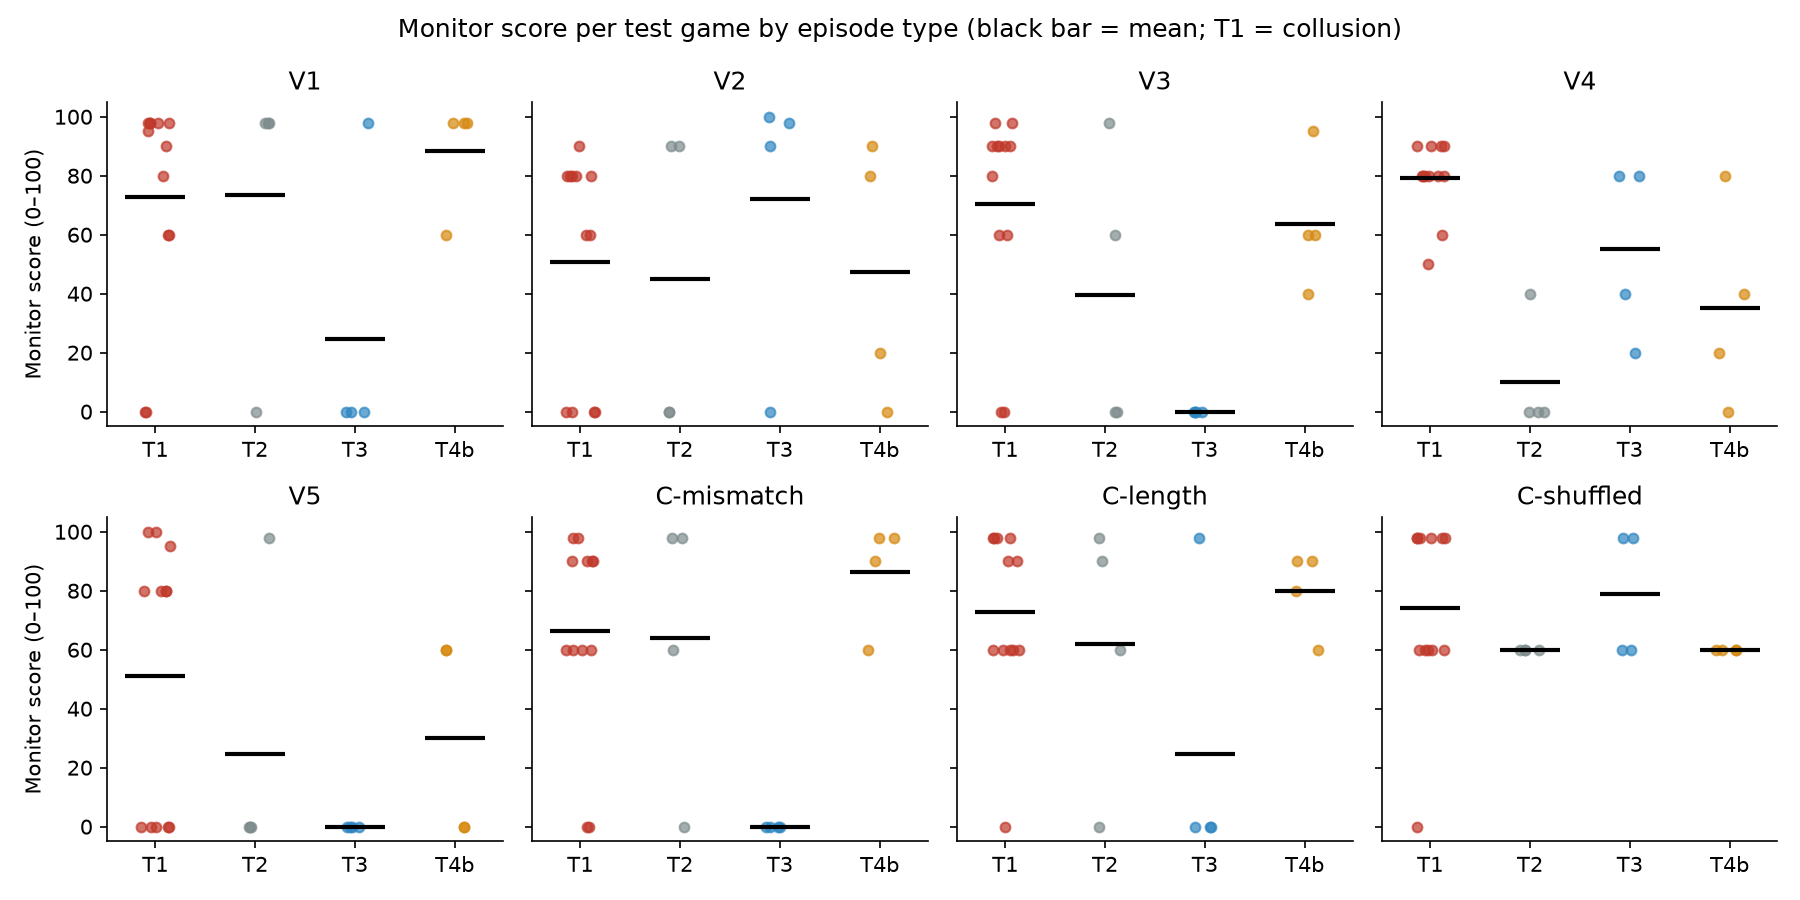
\includegraphics[width=\textwidth]{fig2_per_type_scores_test.png}
\caption{\textbf{Monitor score per test game by episode type} \emph{(exploratory, not pre-registered)}. Each dot is
one test game; the black bar is the type mean (12 Type~1 games, 4 of each negative type). Persona-talk games (T3)
score high in the actions view (V2); same-incentive games (T4b) score highest of all in the messages view (V1).
V4 is the only view where every collusion game (T1) scores above every placebo game (T2).}
\label{fig:pertype}
\end{figure}
% src: figures/captions.md Figure 2.

\subsection{Follow-up 1: pair-order position bias}
Llama gave the top score to the last-listed pair (T-Z) in 21/24 V1 and 17/24 V3 test replies, although T-Z was the
true pair in only 1 of 12 test collusion games. A pre-registered follow-up re-scored the test games with the pair
order randomised (Figure~\ref{fig:followup}). Randomising cut the last-position effect in V1 (21/24 $\rightarrow$
10/24) and V3 (19/24 $\rightarrow$ 9/24) but changed no view's AUROC clearly (V1 +0.017 [$-$0.229, +0.281], V3
+0.042 [$-$0.198, +0.285], V4 $-$0.076 [$-$0.240, +0.111]). The bias is real, but it does not explain the raw-view
failure. With a random order, V4 named the right pair in 8/12 games.
% src: results_22.md §d.2 (R15 §4.6; R16 §4.3); Follow-up 1 row (R16 §4.2, §4.7); RQ8 row (R16 §4.5); captions Fig 7.

\begin{figure}[t]
\centering
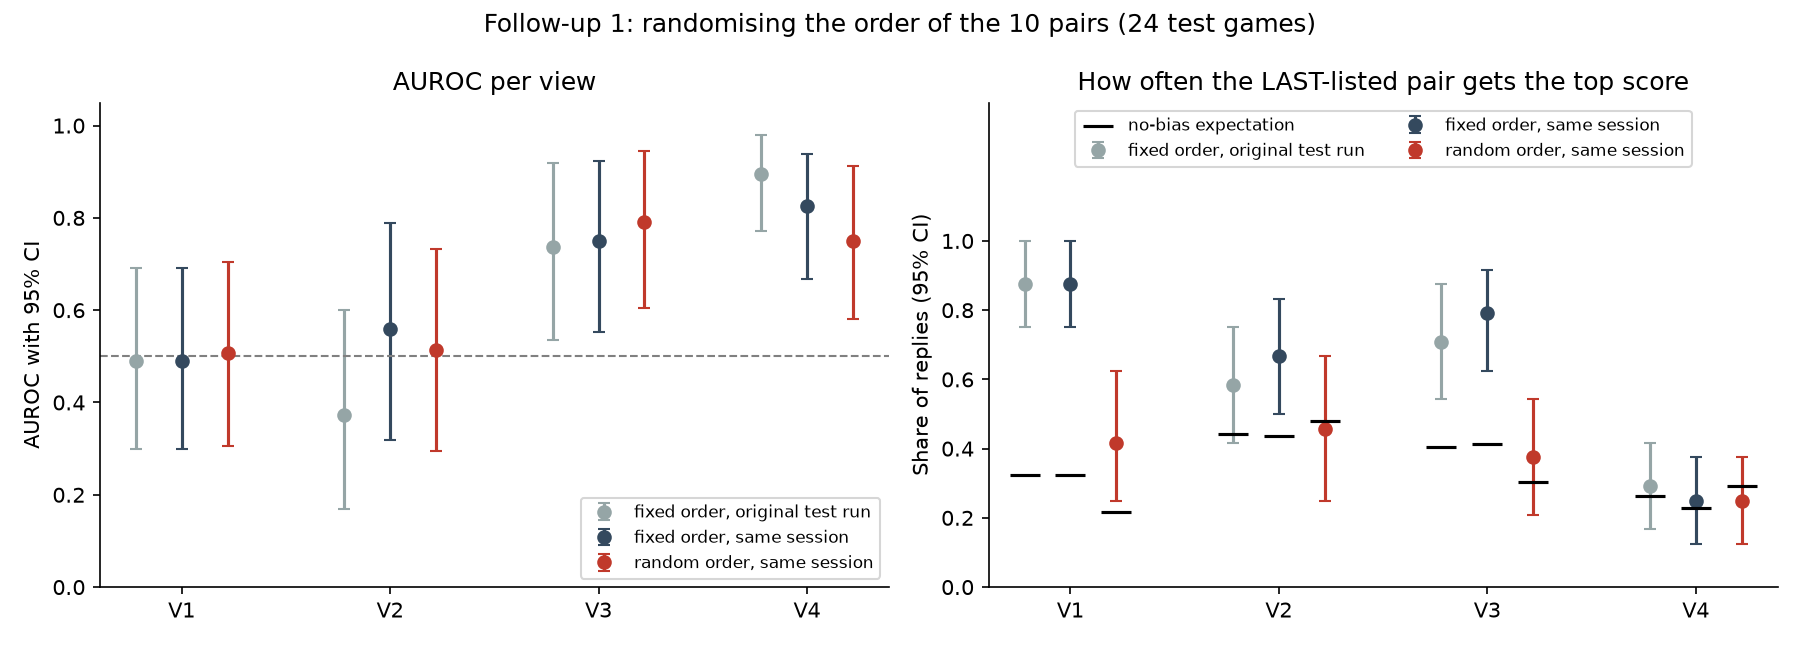
\includegraphics[width=\textwidth]{fig7_pair_order_followup.png}
\caption{\textbf{Follow-up 1: randomising the order of the 10 pairs} \emph{(pre-registered, commit 496fc28)}.
The 24 test games $\times$ V1--V4 were scored in three arms: fixed order in the original test run (grey), fixed
order re-scored in the follow-up session (dark), and a random order per call in the same session (red).
\textbf{Left:} AUROC with 95\% CIs. \textbf{Right:} share of replies in which the last-listed pair gets the top score;
black ticks show the no-bias expectation (allowing for ties). Randomising cuts the last-position effect in V1 and V3
but changes no view's AUROC clearly.}
\label{fig:followup}
\end{figure}
% src: figures/captions.md Figure 7.

\subsection{RQ9: a second monitor model}
The same frozen prompt with \texttt{granite3.3:8b} gave a different ranking (Figure~\ref{fig:granite}): V1 0.729
[0.549, 0.896], V2 0.767 [0.604, 0.917], V3 0.736 [0.573, 0.917] and V4 0.510 [0.292, 0.729] (Kendall $\tau$-b
$-$0.667, a coarse measure with 4 views). Granite showed no last-position preference beyond ties. Granite ran on
different hardware (Apple Metal vs.\ NVIDIA), so model and hardware effects cannot be separated.
% src: results_22.md RQ9 row (R15C §4.2, §4.5, §8).

\begin{figure}[t]
\centering
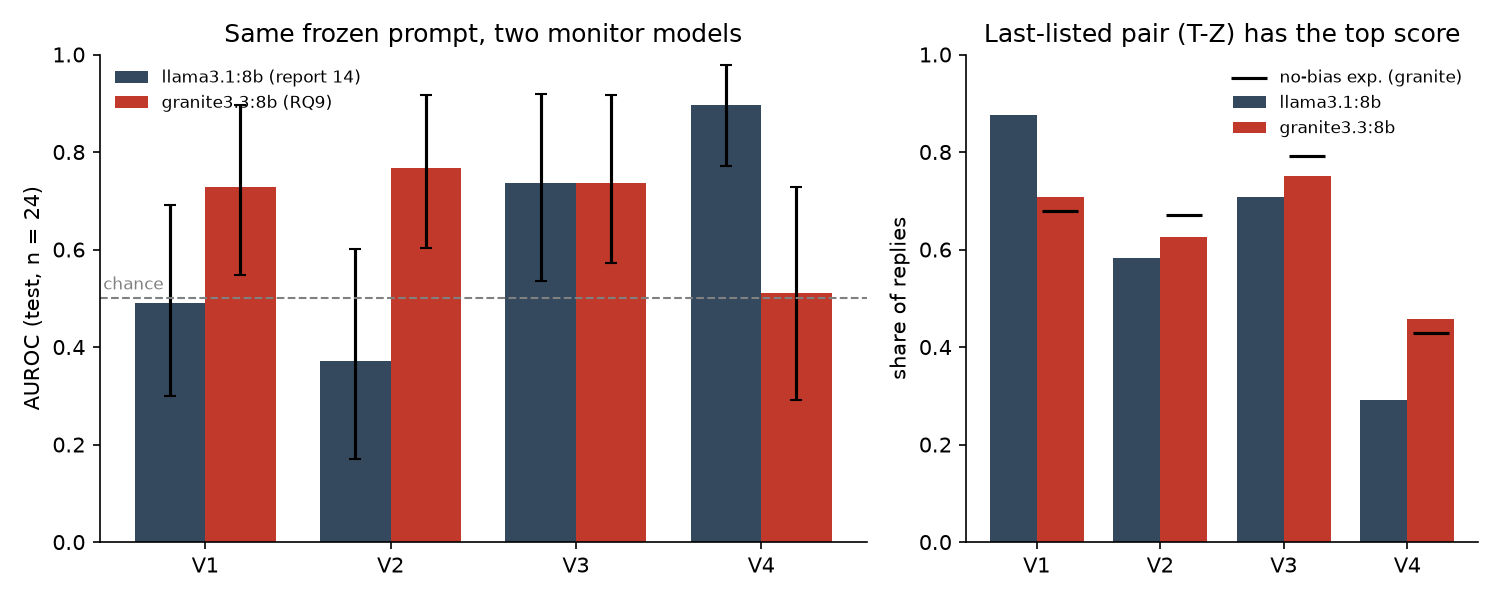
\includegraphics[width=\textwidth]{fig8_rq9_granite.png}
\caption{\textbf{RQ9: the same frozen monitor prompt with a second model} (test set, $n=24$, one sample, one session).
\textbf{Left:} test AUROC per view with 95\% CIs, \texttt{llama3.1:8b} vs.\ \texttt{granite3.3:8b}. The ranking does not
carry over (Kendall $\tau$-b $-$0.67): only V3 is the same (0.736 for both), and V4, best with llama, is at chance
with granite. \textbf{Right:} share of replies in which the last-listed pair (T-Z) has the top score; granite sits at
its no-bias expectation in every view, so the last-position pattern looks specific to llama.}
\label{fig:granite}
\end{figure}
% src: figures/captions.md Figure 8.

\subsection{Pre-registered replication on 48 new games}
Table~\ref{tab:repl22} and Figure~\ref{fig:repl22} give the replication with frozen prompts, one sample and one run
per monitor. There were 0 quality-fail games, so the sensitivity analysis equals the primary. \textbf{Replicated}:
messages alone fail (R1), private plans add nothing (R8), the shuffled control is at chance (R9), and the
model-free capture signal works (R10a), now clearly beating the best LLM view (R10b, +0.264 [0.121, 0.412]).
\textbf{Not replicated}: the structured report's advantages over the raw view (R4) and over a same-length raw view
(R5), and ``persona talk fools actions'' (R7). With llama, ``combining beats actions'' replicated (R3), but only
because llama's action view is below chance (0.324). With granite, the action view was not reliably above chance
(G1), and only llama prefers the structured report (G3). Neither monitor reaches 0.7 on any view of the new games.
% src: results_22.md §g (R21 §4.2, §4.7; R22C §4.4).

\begin{table}[t]
\centering\small
\caption{\textbf{Study 1 replication} (48 new games; frozen \texttt{llama3.1:8b} monitor; granite under amendment~1).
Original column: $n=24$ test. Sources: R21 \S4.7; R22C \S4.4; R14; R15; R15C.}
\label{tab:repl22}
\begin{tabularx}{\textwidth}{@{}lYp{3.7cm}cp{2.3cm}@{}}
\toprule
ID & Hypothesis & Replication [95\% CI] & Original & Outcome\\
\midrule
R1 & Messages alone fail: AUROC(V1) & 0.505 [0.363, 0.655] & 0.490 & confirmed\\
R2 & Structured report works: AUROC(V4) & 0.636 [0.507, 0.751] & 0.896 & confirmed\\
R3 & Combining helps: V3 $-$ V2 & +0.241 [0.063, 0.419] & +0.365 & replicated\\
R4 & Structure beats raw: V4 $-$ V3 & +0.071 [$-$0.128, 0.247] & +0.160 & not replicated\\
R5 & Structure beats same length: V4 $-$ C-length & $-$0.034 [$-$0.212, 0.133] & +0.285 & not confirmed\\
R6 & Same incentive fools messages: V1, T1 vs.\ T4b & 0.495 [0.297, 0.716] & 0.344 & confirmed\\
R7 & Persona fools actions: V2, T1 vs.\ T3 & 0.352 [0.154, 0.578] & 0.219 & not confirmed\\
R8 & Private plans: V5 $-$ V3 & $-$0.022 [$-$0.192, 0.155] & $-$0.031 & no gain again\\
R9 & Shuffled control: AUROC(C-shuffled) & 0.457 [0.315, 0.591] & 0.632 & pass\\
R10a & Code signal: AUROC(capture) & 0.900 [0.811, 0.965] & 0.896 & confirmed\\
R10b & Capture $-$ V4, paired & +0.264 [0.121, 0.412] & --- & capture better\\
\midrule
G1 & Granite action view works: AUROC(V2) & 0.628 [0.488, 0.754] & 0.767 & not confirmed\\
G2 & Granite structured report does not work: AUROC(V4) & 0.582 [0.414, 0.730] & 0.510 & confirmed\\
G3 & Ranking depends on monitor: V4 $-$ V2, llama / granite & +0.313 [0.127, 0.481] / $-$0.046 [$-$0.251, 0.152] & --- & confirmed (mainly llama)\\
G4 & Monitors agree on V3: granite $-$ llama & +0.097 [$-$0.063, 0.262] & --- & no detected difference\\
\bottomrule
\end{tabularx}
\end{table}

\begin{figure}[t]
\centering
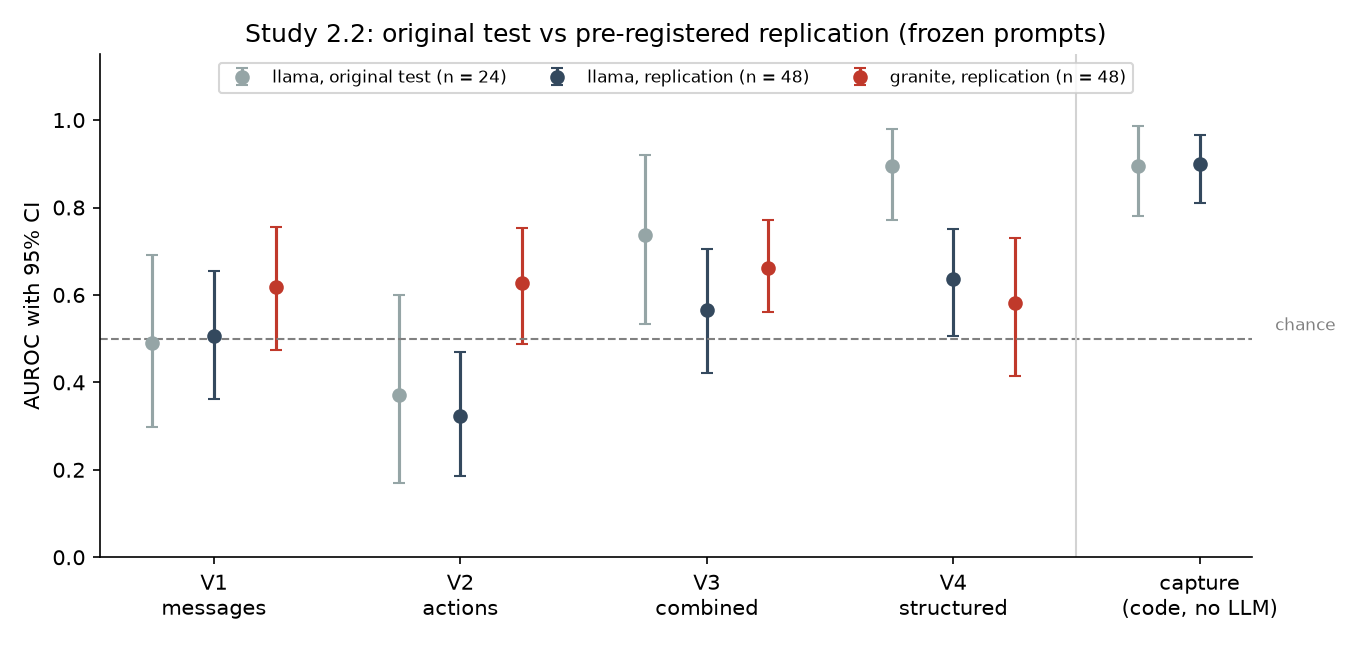
\includegraphics[width=\textwidth]{fig9_replication_22.png}
\caption{\textbf{Study 1: original test vs.\ pre-registered replication} (frozen prompts; one sample per call, one
run per monitor). AUROC with 95\% CIs: llama on the original 24 test games (grey), llama on the 48 replication games
(dark) and granite on the same 48 games (red); the model-free capture signal on the right. The structured report's
original 0.896 shrank to 0.636. No LLM view of either monitor reaches 0.7 on the new games, while capture stays at
about 0.90. V5 and the C-length / C-mismatch controls are not shown (no replication AUROC reported).}
\label{fig:repl22}
\end{figure}
% src: figures/captions.md Figure 9.

% ====================================================================================
\section{Results: Study 2 (standard of evidence)}
\label{sec:23}

\textbf{Single families (test, $n=24$; Table~\ref{tab:rules}).} Talk alone is not evidence: the judge flagged 11 of 12
innocent games and ranked below chance (0.396). Outcomes alone rank games well, but the shared-incentive lookalike
fools them: coalition gain (R2, 0.872 [0.736, 0.986]) and capture (0.896, exploratory) each flag 2 of 4 Type~4b
games. Dependence alone is weaker, undefined in 3 games, and fooled by every lookalike type at least once.

\begin{table}[t]
\centering\footnotesize\setlength{\tabcolsep}{4pt}
\caption{\textbf{Frozen decision rules on the 24 test games} (12 collusion; 4 per lookalike type) and their
replication AUROC (48 new games). Counts are games flagged at the frozen thresholds. R4 and R5 are binary rules
(no AUROC). Sources: results\_23.md \S1, \S2, \S6 (17C; R22C \S4.2); capture: R15 \S4.4, counts R17C \S4.5.}
\label{tab:rules}
\begin{tabular}{@{}lccccccc@{}}
\toprule
Rule & AUROC test & TPR & FPR & T2 & T3 & T4b & AUROC replication\\
\midrule
R1 judge (talk only)        & 0.396 [0.205, 0.597] & 8/12 & 11/12 & 4/4 & 4/4 & 3/4 & 0.543 [0.392, 0.693]\\
R2 coalition gain           & \textbf{0.872} [0.736, 0.986] & 10/12 & 2/12 & 0/4 & 0/4 & 2/4 & \textbf{0.885} [0.786, 0.961]\\
R3 dependence ($n=21$)      & 0.736 [0.491, 0.942] & 9/12 & 4/12 & 1/4 & 1/4 & 2/4 & 0.682 [0.518, 0.823]\\
capture (exploratory)       & 0.896 [0.781, 0.986] & 8/12 & 2/12 & 0/4 & 0/4 & 2/4 & 0.900 [0.811, 0.965]\\
\midrule
R4 legal style              & ---  & 2/12 & 0/12 & 0/4 & 0/4 & 0/4 & ---\\
R5 gain AND dependence      & ---  & 4/12 & 2/12 & 0/4 & 0/4 & 2/4 & ---\\
R6 points                   & 0.792 [0.667, 0.917] & 11/12 & 4/12 & 1/4 & 0/4 & 3/4 & 0.826 [0.721, 0.920]\\
R7 learned (logistic)       & 0.812 [0.611, 0.972] & 10/12 & 2/12 & 0/4 & 0/4 & 2/4 & 0.844 [0.722, 0.941]\\
\bottomrule
\end{tabular}
\end{table}
% src: results_23.md §1 and §2 tables; §6 "All rules on the replication" (R3 n = 47 on replication); capture replication = R21 R10a.

\textbf{Combining did not help (RQ-E3).} The pre-registered comparison of the best combined rule (R6) with the best
single family (R2), both chosen on dev, was $-$0.080 [$-$0.208, 0.045]: no clear difference. Ablations show why:
almost all of the signal comes from coalition gain. Removing gain cost R6 +0.292 [0.125, 0.458] and R7 +0.375
[0.111, 0.639] of AUROC, while removing the judge, dependence or word--action consistency changed little. Word--action
consistency (RQ-E5) was a null: removing it changed R6 by 0.000 and R7 by $-$0.062, both CIs including 0.
% src: results_23.md §2 (RQ-E3, ablation table).

\textbf{The plus-factor rule.} An exploratory rule (post hoc, motivated by report 15) flags a game only if it shows
parallel conduct (capture $\geq$ 0.625) \emph{and} coordination words ($C_{\text{kw}} \geq$ 0.7375), both thresholds
set on dev. It removed every false positive, including both shared-incentive games, but caught only 1 of 12 real
collusion games. The frozen legal-style rule R4 shows the same trade-off: 0 false positives, 2/12 caught.
% src: results_23.md §4.

\textbf{Replication (Figure~\ref{fig:repl23}).} The frozen judge and rules file were applied once to the 48 new games.
E1 (gain works) was confirmed, 0.885 [0.786, 0.961]; E2 (the talk-only judge is near chance) was confirmed,
0.543 [0.392, 0.693]; E3 (R6 $-$ R2) was not replicated, $-$0.059 [$-$0.135, 0.010], and nor was the secondary E3b
(R7 $-$ R2, $-$0.042 [$-$0.155, 0.067]). The shared-incentive lookalike stayed the hardest case: gain flagged 3/8 of
those games, against 1/8 placebo and 1/8 persona games. The plus-factor rule caught 0/24 colluders with 0/24 false
positives.
% src: results_23.md §6 (R22C §4.2).

\begin{figure}[t]
\centering
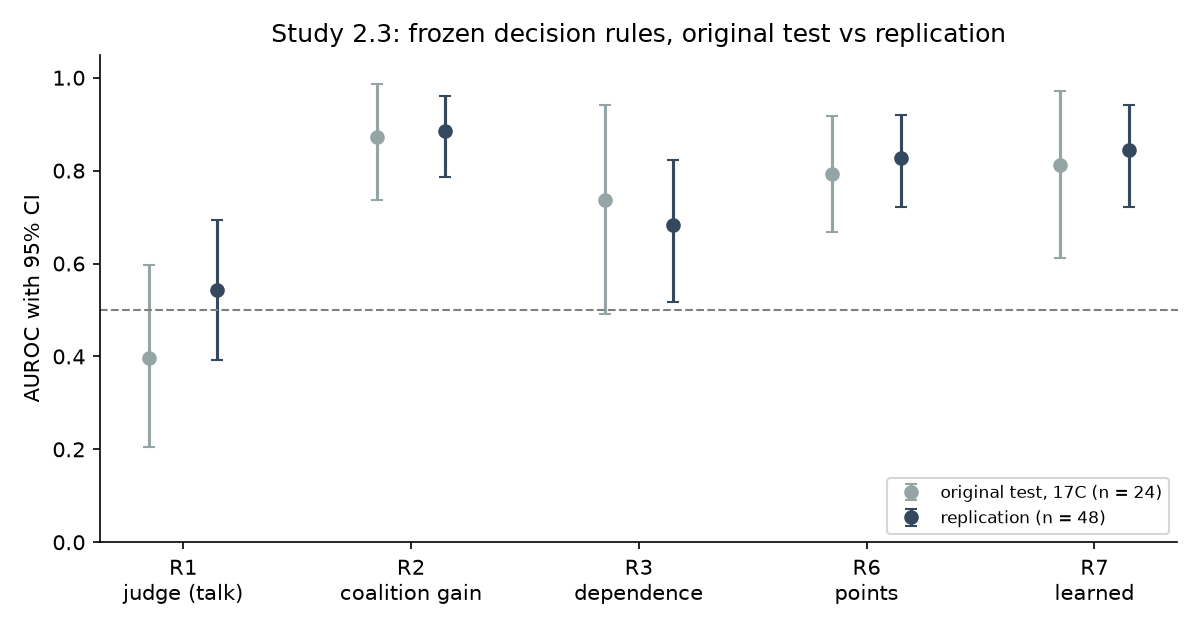
\includegraphics[width=0.92\textwidth]{fig10_replication_23.png}
\caption{\textbf{Study 2: frozen decision rules, original test vs.\ replication} (pre-registered; frozen rules, not
refit; one judge sample). AUROC with 95\% CIs on the 24 original test games (grey) and the 48 replication games (dark).
The gain rule R2 replicates (0.872 $\rightarrow$ 0.885), and the talk-only judge R1 stays near chance (0.396
$\rightarrow$ 0.543). The combined rules R6 and R7 do not beat R2. R4 and R5 are binary and have no AUROC.}
\label{fig:repl23}
\end{figure}
% src: figures/captions.md Figure 10.

\textbf{Our standard of evidence.} Outcome evidence (gain, capture) is necessary and replicates, but it is not
sufficient against a shared incentive. None of the communication evidence we measured was a usable plus factor:
requiring it removes false positives only by missing most real collusion.
% src: results_23.md §6 "Final standard of evidence".

% ====================================================================================
\section{Failure Modes of LLM Monitors}
\label{sec:failures}

\begin{enumerate}
  \item \textbf{Constant-score collapse.} The single-score format (one 0--100 score per game) returned 80 in 96/96 dev
  calls, and it was ruled ineligible on dev before any test call. Scoring each pair instead gave 4--10 distinct values
  per view.
  % src: results_22.md §d.1 (R13 §0, §2).
  \item \textbf{Judge ceiling.} The messages-only judge gave almost every game a top pair score near 98 and never scored
  a pair above 98 (0 of 480 pair scores). Because E1's frozen plus threshold was ``above 98'', E1 could never add a point
  in R6. Its top pair was the true pair in only 2 of 12 collusion games, and it gave the top score to the last-listed
  pair T-Z in 18 of 24 test games.
  % src: results_23.md §3.
  \item \textbf{Position bias (llama only).} On the replication, the last-listed pair had llama's top score in 44/48 V1
  replies (no-bias expectation 0.215), 44/48 V3 and 48/48 C-shuffled replies; granite showed no preference beyond ties.
  The bias changes \emph{who} is named, not \emph{how well} games are ranked (Follow-up~1).
  % src: results_22.md §d.2 (R21 §4.8; R22C §4.4; R16 §5).
  \item \textbf{Session effect.} Within one Ollama session, repeats were identical. Between sessions, V2 re-scored
  unchanged went from 0.372 to 0.559 AUROC (+0.188 [+0.007, +0.389]; mean absolute difference 10.79, Spearman 0.653).
  % src: results_22.md §d.3 (R13 §4; R16 §4.2, §4.4).
  \item \textbf{Small-sample optimism.} Best first results shrank on new games: llama V4 0.896 $\rightarrow$ 0.636 and
  granite V2 0.767 $\rightarrow$ 0.628. Between dev and test, V3 moved from 0.319 to 0.736 (+0.417 [0.142, 0.684]),
  and the view rankings agreed only weakly (Kendall $\tau$ 0.255).
  % src: results_22.md §a "Small-sample optimism"; §e (R15 §4.1).
  \item \textbf{Reading friendly talk as a pair signal.} V4 at its frozen threshold flagged all 8 persona games on the
  replication (2/4 on the original test). Its mention-count lines make friendly talk look like coordination. In one
  persona game where nobody ever went to the bar, the V4 monitor scored 80 and wrote: ``T and Z repeatedly mention each
  other in messages, suggesting coordination.''
  % src: results_22.md §d.6 (R21 §4.8; R14 §4.4); excerpts_22.md case (d).
\end{enumerate}

% ====================================================================================
\section{Discussion and Limitations}

\textbf{What this means for auditing multi-agent systems.} In our setting, \emph{what agents did} carried the signal and
\emph{what an 8B model concluded from reading the record} did not. A simple code signal (capture) replicated at
about 0.90, while every LLM view of both monitors lay between 0.32 and 0.66 on new games, and the best LLM view on the
first test did not survive. An auditor of agent systems should treat model-free behaviour statistics as the baseline that
any LLM monitor must beat, report LLM monitor results per model, and expect LLM verdicts to move with the model, the
prompt order and the session.

\textbf{The link to antitrust.} Our data reproduce the first half of the plus-factor doctrine clearly: parallel conduct
and coalition gain are the strongest single evidence, yet they also flag agents that merely share an incentive (gain
flagged 3/8 shared-incentive games on the replication). The second half did not work here: neither keyword evidence nor an
LLM judge of the public talk was a usable plus factor, because agents in this game talk about coordinating all the time,
honest ones included. Real cartels rarely announce their agreement in public, and an auditor, like a competition
authority, will often lack the private channel. Our results suggest that without such private evidence, the honest
verdict on a ``shared incentive'' pattern is ``parallel conduct, agreement not shown''.

\subsection*{Limitations}
\begin{itemize}
  \item \textbf{Small samples.} 24 test and 48 replication games, with 8 or fewer per lookalike type; one false positive moves
  a type's rate by 25 points on test and 12.5 points on the replication, and most CIs are wide.
  \item \textbf{Narrow setup.} One game (El Farol), one agent model (\texttt{qwen2.5:7b}), 8 rounds. The collusion is suggested
  by a prompt (the alliance note proposes the plan), not invented by the agents, and it is not fully secret (6.5\% of
  focal public messages reveal joint action).
  \item \textbf{Two small monitors} (8B), one frozen prompt format and one sample per call. Scores can change between
  sessions, and the second monitor ran on different hardware, so model and hardware are confounded.
  \item \textbf{An unplanned clue.} Shared-incentive agents talk about their ``deposit'' in public, and the flag-only
  cleaner leaves it visible to monitors.
  \item \textbf{Data quality.} 1.75\% of generation calls failed (all truncation) and their rounds are excluded; 1 persona
  game partly behaved like collusion and 2 shared-incentive games did not follow the incentive (labels stay as configured).
  \item \textbf{Degenerate thresholds.} V1, V3 and C-mismatch had a frozen threshold of 0 (flag everything), so their
  threshold metrics carry no information.
  \item \textbf{V2 instability.} V2 failed the stability gate (RQ0.4), so V2-based results (including RQ2) carry this
  caveat.
  \item \textbf{Exploratory parts.} Code-signal comparisons beyond Dep and the plus-factor rule were not pre-registered;
  pooled results include dev selection data; the uptake rule~v2 was developed on pilot~1 and confirmed on pilot~2 only.
  \item \textbf{In-sample dev fits.} Thresholds and rule choices come from 24 dev games, so dev performance overstated test
  performance (e.g.\ R2's balanced accuracy 0.958 on dev vs.\ 0.833 on test).
  \item \textbf{One judge} (\texttt{llama3.1:8b}, one sample, one session) with a fixed pair order that likely biases its
  pair choice.
\end{itemize}
% src: results_summary.md "Main limitations"; results_22.md §e; results_23.md §5.

\subsection*{Future Work}
\begin{enumerate}
  \item Larger test sets with more games per lookalike type, so that primary comparisons such as RQ2 and RQ5 can be settled.
  \item Score several sessions per view and report the between-session spread, especially for V2 and V4.
  \item Make randomised pair and agent order the default monitor format, with an explicit ``no pair'' option to reduce ties.
  \item Treat simple action signals (coGO, capture, $G_{\text{others}}$) as required baselines, and test a combined
  code + LLM rule on dev first.
  \item Remove the shared-incentive ``deposit'' clue at generation time, so that lookalike tests behaviour only.
  \item Test emergent (not prompted) collusion, other games and larger monitors.
\end{enumerate}
% src: results_22.md §e "What we would do next" (items 2-6); item 6 from the listed limitations.

% ====================================================================================
\section{Conclusion}

We built a pre-registered, fully local testbed for auditing collusion between LLM agents, with lookalikes that target
word evidence and outcome evidence separately, and we re-tested every frozen choice on 48 new games. The result is a
clear ordering of evidence: model-free behaviour signals (capture, coalition gain) were the most reliable and they
replicated; small LLM monitors were mediocre, model-dependent and unstable, and their best first result did not hold;
messages alone and talk-only judging stayed near chance; and combining evidence did not beat gain alone.

For the standard of evidence, our data agree with the antitrust intuition: parallel conduct and coalition gain are
necessary signals but not proof, because a shared incentive produces the same outcomes. In this setting no
communication evidence we measured could serve as the plus factor. Detecting the agreement itself, as opposed to
its consequences, remains open.

% ====================================================================================
\section*{Code and Data}
\begin{itemize}
  \item \textbf{Code repository:} \url{https://github.com/AyushSingh110/collusion-evidence-lab} (pre-registrations in
  \texttt{configs/}, per-task reports in \texttt{notes/reports/}, results in \texttt{writeup/}).
  \item \textbf{Data:} games, views, monitor outputs and the full LLM cache are kept out of git (\texttt{data/},
  \texttt{runs/}, \texttt{cache/}); every report gives the commands that produced it. Without the cache, re-running makes
  new model calls, which may not reproduce every score exactly (session nondeterminism).
  \item \textbf{Info-hazards:} none beyond the general topic; the collusion is a prompted toy behaviour in a bar game.
\end{itemize}

\section*{Author Contributions}
[Author 1] led the project, research design and evaluation. [Author 2] built the metrics, evidence signals, decision
rules and statistics. [Author 3] built the harness integration, data pipeline, views, runners and caching. All authors
reviewed the final manuscript. \emph{(Replace with your names and roles.)}

% ------------------------------------------------------------------ references
\begin{thebibliography}{99}\small
\bibitem{shi2026} Shi, Zhang, Sch\"olkopf, Conitzer and Jin (2026). \emph{When Agents Lie: Premeditation, Persistence, and
Exploitation in Repeated Games.} arXiv:2607.05132. Code: \url{https://github.com/Jerick-1380/LLM-Trust-Breaking}.
\bibitem{nguyen2026} Nguyen et al. (2026). \emph{TraceGuard: Structured Multi-Dimensional Monitoring as a
Collusion-Resistant Control Protocol.} arXiv:2604.03968.
\bibitem{nakamura2026} Nakamura et al. (2026). \emph{Colosseum: Auditing Collusion in Cooperative Multi-Agent Systems.}
arXiv:2602.15198.
\bibitem{fish2024} Fish et al. (2024). \emph{Algorithmic Collusion by Large Language Models.} arXiv:2404.00806.
\bibitem{agrawal2025} Agrawal et al. (2025). \emph{Evaluating LLM Agent Collusion in Double Auctions.} arXiv:2507.01413.
\bibitem{mathew2024} Mathew et al. (2024). \emph{Hidden in Plain Text: Emergence and Mitigation of Steganographic
Collusion in LLMs.} arXiv:2410.03768.
\bibitem{tailor2025} Tailor (2025). \emph{Audit the Whisper: Detecting Steganographic Collusion in Multi-Agent LLMs.}
arXiv:2510.04303.
\bibitem{kovacic2011} Kovacic, Marshall, Marshall and Raiff (2011). Plus Factors and Agreement in Antitrust Law.
\emph{Michigan Law Review} 110(3).
\bibitem{twombly2007} \emph{Bell Atlantic Corp.\ v.\ Twombly}, 550 U.S. 544 (2007).
\bibitem{theatre1954} \emph{Theatre Enterprises, Inc.\ v.\ Paramount Film Distributing Corp.}, 346 U.S. 537 (1954).
\bibitem{arthur1994} Arthur (1994). Inductive Reasoning and Bounded Rationality. \emph{American Economic Review} 84(2),
406--411.
\end{thebibliography}

% ====================================================================================
\appendix
\section{Deviations from the pre-registrations}
\label{app:dev}
{\footnotesize
Items 1--12 are from report 10 \S B4; items 13 onward were added later; items 23 onward are the RQ9 / replication phase.
``When'' says whether the deviation was decided before or after the related data. Source: \texttt{writeup/results\_22.md} \S f.
\setlength{\tabcolsep}{3pt}
\begin{longtable}{@{}p{0.03\textwidth}p{0.36\textwidth}p{0.27\textwidth}p{0.29\textwidth}@{}}
\toprule
\# & What & Why & When (relative to the related data)\\
\midrule
\endfirsthead
\toprule
\# & What & Why & When (relative to the related data)\\
\midrule
\endhead
\bottomrule
\endfoot
1 & Pre-freeze changes: possessive name pattern, hint folded into alliance\_v3, placebo\_v3, 2 machines & rule bug; b2 at risk; length match; machine C unavailable & before any pilot data (the hint was motivated by 3 earlier smoke games)\\
2 & Freeze commit 84fca68 $\rightarrow$ 4909c7e & the title still said DRAFT & before pilot 1\\
3 & Pilots 1 and 2 on machine B only (prereg: A and B) & operational & before the data; no design change\\
4 & Departure from U1 $\rightarrow$ Amendment 1 (language line, uptake rule v2, pilot 2, new gate) & U1 targeted a cause that was not observed; the rule missed real coordination; language drift & \textbf{after pilot-1 data} (rule v2 tested on new data, pilot 2)\\
5 & Pilot-1 hand-check made descriptive & the rule had been replaced; two raters for reliability & after pilot-1 data, before the hand-check was filled\\
6 & E2 = 10 rounds instead of 12 & lead's decision & after pilot 1; moot\\
7 & Cleaner becomes flag-only (except 8-word copies and header phrases) & over-removal concern; Type 4b ``deposit'' talk is behaviour & after pilot 1\\
8 & Language line (``English only'') & language drift in pilot 1 & after pilot 1\\
9 & Amendment 1 committed together with code, not alone & --- & before pilot 2\\
10 & Secrecy variant v4 + 2-game re-pilot & executes frozen \S5 (reveal rate 12.5\%) & after pilot-2 data; recorded before its own calls\\
11 & Proceed with v4 although the re-pilot reveal rate stayed 12.5\% & frozen \S5 sets no further target & after the re-pilot data\\
12 & Repair re-ask not used & keep all failures as data & after the pilot-2 failures\\
13 & RQ0.2 criteria operationalised (e.g.\ ``persona talk'' = names the partner + a warm word) & the frozen text gave no exact rule & stated in the script before computing RQ0.2\\
14 & Erratum and analysis decisions: alternation shows in G\_others only; C\_kw = literal sum of both directions; tie rules; threshold candidates = observed dev scores & correctness of the amendment's explanation; rules not pre-registered & \textbf{before any monitor result}\\
15 & num\_ctx 16384 for all monitor calls (new manifests, same templates) & every V5 view exceeded the 8192 guard & after the views were rendered, \textbf{before any monitor call}\\
16 & Format eligibility clause: a constant-score format is ineligible, so v3\_pairs was chosen & v1 gave 80 on 96/96 dev calls & \textbf{after dev monitor data, before any test call}\\
17 & \texttt{analyse\_22.py --freeze-extra} (adds keys to the frozen file without overwriting) & record format, digest and RQ0.3 / RQ0.4 in the frozen file & before the test run\\
18 & Test-analysis addendum: ``degenerate threshold'' labels; supplementary per-type AUROC for RQ3; RQ2 caveat; exploratory C-length $-$ V3 & three views had threshold 0 & \textbf{before test scoring}\\
19 & Exploratory robustness analyses, plus an unplanned position-bias check & robustness; prompted by an excerpt & \textbf{after test data}; labelled exploratory\\
20 & Follow-up 1 pre-registered, with a same-session control arm added before the commit & test the position-bias explanation & after test data, \textbf{before any follow-up call}\\
21 & Follow-up random arm also uses sample\_idx 1 (same seed as the control arm) & the arms then differ only in pair order & before any follow-up call\\
22 & Documentation corrections: section reference ``report 15 \S6'' $\rightarrow$ \S4.6 & typo & no data involved\\
23 & RQ9 granite run recorded machine id \texttt{m\_5acffc7a} instead of \texttt{C}; cache shard kept as is; fixed for later runs & environment variable not loaded in the tool shell & \textbf{after} the RQ9 run; provenance only, results unaffected (pinned digest checked on every call)\\
24 & RQ9 run paused at 11/96 calls to ask the lead's OK; the kill removed the first session's manifest record & time limit (Rule H) & during the run; nothing re-scored\\
25 & The RQ9 granite manifest adds a \texttt{model\_digest} field & record the digest in the config & before the RQ9 run\\
26 & E3 fixed as primary (best single R2 vs.\ best combined R6; tie broken by the lower rule number); E3b = R7 $-$ R2 added as secondary & no 17C record existed when the prereg was drafted & \textbf{before any replication game}\\
27 & Replication labels in a separate file; C-mismatch partners within type across all 48 games; full outcome map for every rule; primary = all games, sensitivity = without quality-fail games & never touch the original labels / split; avoid undefined outcomes & \textbf{before any replication game}\\
28 & The labels writer refuses to overwrite even an identical file & stricter, as the task asked & before generation\\
29 & Outcome words for ``otherwise'' branches; last-position-max with a tie-aware expectation; quality-file format & the prereg gave ``otherwise'' or no format & \textbf{before any replication output}\\
30 & Amendment 1 (granite): full outcome map for G2; G4 note ``no detected difference, not equivalence''; analysis refuses frozen dev game ids & avoid undefined outcomes and over-reading & \textbf{before any replication data}\\
31 & G1--G4 code checks each monitor line by \texttt{prompt\_sha256}; ``undetermined (no CI)''; a G3 / G4 zero estimate counts as ``not confirmed'' & the amendment did not cover these cases & \textbf{before any replication monitor output}\\
32 & \texttt{g\_ec16a9027c}: G\_others = 2.2e-16 counted as $>0$ by the frozen rule; effect check reported both ways (24/24 by rule, 23/24 substantively) & float artefact in a descriptive check & \textbf{after} the generation data; descriptive only\\
33 & Replication quality and view checks run with path-only copies of the task-12 scripts (diff-checked) & keep report 12's definitions exactly & before the monitor run\\
34 & Report 21 gives V2 / V3 replication point estimates derived by subtraction (no CI) & context for R3 / R4 & after the analysis; descriptive\\
35 & Granite-only replication measures not computed before the llama file arrived & keep the single G1--G4 run the first look & before the G1--G4 run\\
36 & The llama V1--V4 subset of machine B's 384-line file selected by the \texttt{view} field only; lines copied byte for byte & amendment 1 specifies ``the V1--V4 subset'' & \textbf{after} the data existed; score-blind, recorded before the G1--G4 run\\
37 & Final-results documentation: ``position bias explains the raw-view failure'' keeps NOT SUPPORTED; Figure 10's 17C values copied from report 17C; Figure 9 omits V5 and two controls & stay within reported numbers & after all data; documentation only\\
38 & Final labels reworded: ``actions alone fail'' $\rightarrow$ ``REPLICATED (llama); borderline for granite''; ``view ranking depends on the monitor'' $\rightarrow$ ``NOT SHARED BETWEEN MONITORS (G3; rests mainly on llama)'' & precision of wording & after all data; wording only, no number changed\\
39 & Documentation repairs: merge-conflict markers in the DEVLOG removed with both sides kept; two citation-section fixes from the number audit & merge artefacts; audit findings & no data involved\\
\end{longtable}
}

\section{Reproducibility}
\label{app:repro}
{\small
\begin{tabularx}{\textwidth}{@{}lllY@{}}
\toprule
Document & Commit & LF sha256 (first 16) & Status relative to data\\
\midrule
Frozen RQ0.1 pre-registration & 4909c7e & c5976220465c10f5 & before pilot 1\\
Amendment 1 & 2d47580 & c214284753ff2cf1 & after pilot-1 data, before pilot 2\\
Amendment 2 & a989c7a & ccb24bbe99095b88 & before any dataset game\\
Erratum to Amendment 2 & 0dfd1b1 & ef31afca9c45d630 & before any monitor result; changes no rule\\
Frozen monitor (\texttt{monitor\_frozen.json}) & 89bdb79 & ccc4bf07838be73e & before any test call\\
Follow-up 1 pre-registration & 496fc28 & 0d6aaa412b394419 & before any follow-up call\\
Replication pre-registration & 2bc3d3a & d9d25b583b1d6052 & before any replication game existed\\
Replication amendment 1 (granite) & 306502e & 778cf66b03bdea1f & before any replication view was rendered\\
\bottomrule
\end{tabularx}
\par\medskip
\textbf{Frozen inputs for the replication:} llama monitor 89bdb79; Study 2 judge and rules 404f356 (rules file sha256
\texttt{ce0b8840\ldots}); granite manifest 57206cb. \textbf{Models} (Ollama 0.40.3, pinned by digest in
\texttt{configs/pins.json}): \texttt{qwen2.5:7b} \texttt{845dbda0ea48\ldots}, \texttt{llama3.1:8b} \texttt{46e0c10c039e\ldots},
\texttt{granite3.3:8b} \texttt{fd429f23b909\ldots}. Seeds: dataset 20261023, pilots 20261024 / 20261025, re-pilot 20261026,
replication 20261027; bootstrap seed 20261023. The final write-up corresponds to repository commit \texttt{dc64f31}.
\par\medskip
\textbf{How to run} (one conda environment, \texttt{collusion-lab}):
\begin{verbatim}
conda env create -f environment.yml
conda run -n collusion-lab pytest -q                    # mock transport, no model calls
conda run -n collusion-lab python scripts/check_env.py  # Ollama 0.40.3 + pinned digests
conda run -n collusion-lab python scripts/make_plan.py --name <plan> --seed <seed> \
    --counts 1=24 2=8 3=8 4=8 --machines A B --rounds 8
conda run -n collusion-lab python -u scripts/run_plan.py --plan configs/plans/<plan>.json
conda run -n collusion-lab python scripts/merge_check.py --plan configs/plans/<plan>.json \
    --raw-dir data/raw/<plan>
\end{verbatim}
The per-task reports in \texttt{notes/reports/} list the exact rendering, monitor and analysis commands.
}

\section*{LLM Usage Statement}
We used Claude (Anthropic), through Claude Code, as an engineering assistant: it wrote and tested most of the code
under our instructions, ran the local experiments, drafted the per-task reports and drafted this paper from our
write-up files. All design decisions were made by the team. Every number in this paper is copied from the project's
reports, each traceable to a report section, and the team verified the claims.

\end{document}
